\documentclass{article}
\usepackage[utf8]{inputenc}

\title{CSC263: Problem Set 8}
\date{December 3, 2019}

\usepackage[utf8]{inputenc}
\usepackage{graphicx}
\usepackage{listings}
\usepackage{xcolor}
\usepackage{natbib}
\usepackage{graphicx}
\usepackage{amsmath}
\usepackage{enumitem}
\usepackage{mathtools}

\definecolor{codegreen}{rgb}{0,0.6,0}
\definecolor{codegray}{rgb}{0.5,0.5,0.5}
\definecolor{codepurple}{rgb}{0.58,0,0.82}
\definecolor{backcolour}{rgb}{0.95,0.95,0.92}

\DeclarePairedDelimiter\floor{\lfloor}{\rfloor}


\lstdefinestyle{mystyle}{
    backgroundcolor=\color{backcolour},   
    commentstyle=\color{codegreen},
    keywordstyle=\color{magenta},
    numberstyle=\tiny\color{codegray},
    stringstyle=\color{codepurple},
    basicstyle=\ttfamily\footnotesize,
    breakatwhitespace=false,         
    breaklines=true,                 
    captionpos=b,                    
    keepspaces=true,                 
    numbers=left,                    
    numbersep=5pt,                  
    showspaces=false,                
    showstringspaces=false,
    showtabs=false,                  
    tabsize=2
}
 
\lstset{style=mystyle}

\begin{document}

\maketitle

\section{Problem 2}

\begin{enumerate}[label=(\alph*)]

\item The running time of breadth first search would be $O(n^2)$, where $n$ is the number of vertices in the graph $K_n$. From page 597 BFS runs in $O(|V| + |E|)$ which is equal to $O(n + |E|)$ in this case. But note that $K_n$ is a complete graph, which means each vertex in $K_n$ has a degree of $n-1$. As there are $n$ vertices with each having a degree of $n-1$, there are $n(n-1)$ edges. So we can replace $|E|$ with $n(n-1)$ so then $O(n + |E|)$ = $O(n + n(n-1))$ = $O(n + n^2 - n)$ = $O(n^2)$. 

\item
\begin{lstlisting}[language=Python]
BFS_Connected(G,s): #(Original code from Page 595)
    for each vertex u in  G.V - {s}
        u.color D WHITE
        u.d = 1
        u.pi = NIL
    s.color = GRAY
    s.d = 0
    s.pi = NIL
    Q = NIL (empty set)
    ENQUEUE(Q,s)
    count = 1
    first_iteration = True
    while not Q.empty:
        u = DEQUEUE(Q)
        for each v in G.Adj[u]
            if v.color == WHITE
                v.color D GRAY
                v.d = u.d + 1
                v.pi = u
                count += 1
                ENQUEUE(Q,v)
        u.color = BLACK
        if count == len(G.V) && first_iteration:
            return True
        first_iteration = False
    if count == len(G.V):
        return True
    return False
\end{lstlisting}
This algorithm work as $k_n$ is a complete graph then that means that every vertex has an edge to all the other vertices. So to see if a graph is complete, we check that all vertices have $n-1$ edges.

\item The disconnected graph below will take $\theta(n^2)$ time, assuming that we start on a vertex that is connected. This is due to the fact that the while loop will keep iterating as line 23 will never be true since it is impossible to reach all the vertices. So the algorithm will go to n-1 vertices and (n-1)(n-2) edges (since there are 4 vertices that are connected and each of those vertices have n-2 edges since they also cannot reach vertex E). This is because the BFS will not stop until all it goes through all the vertices and its edges.


\begin{figure}[htp]
    \centering
    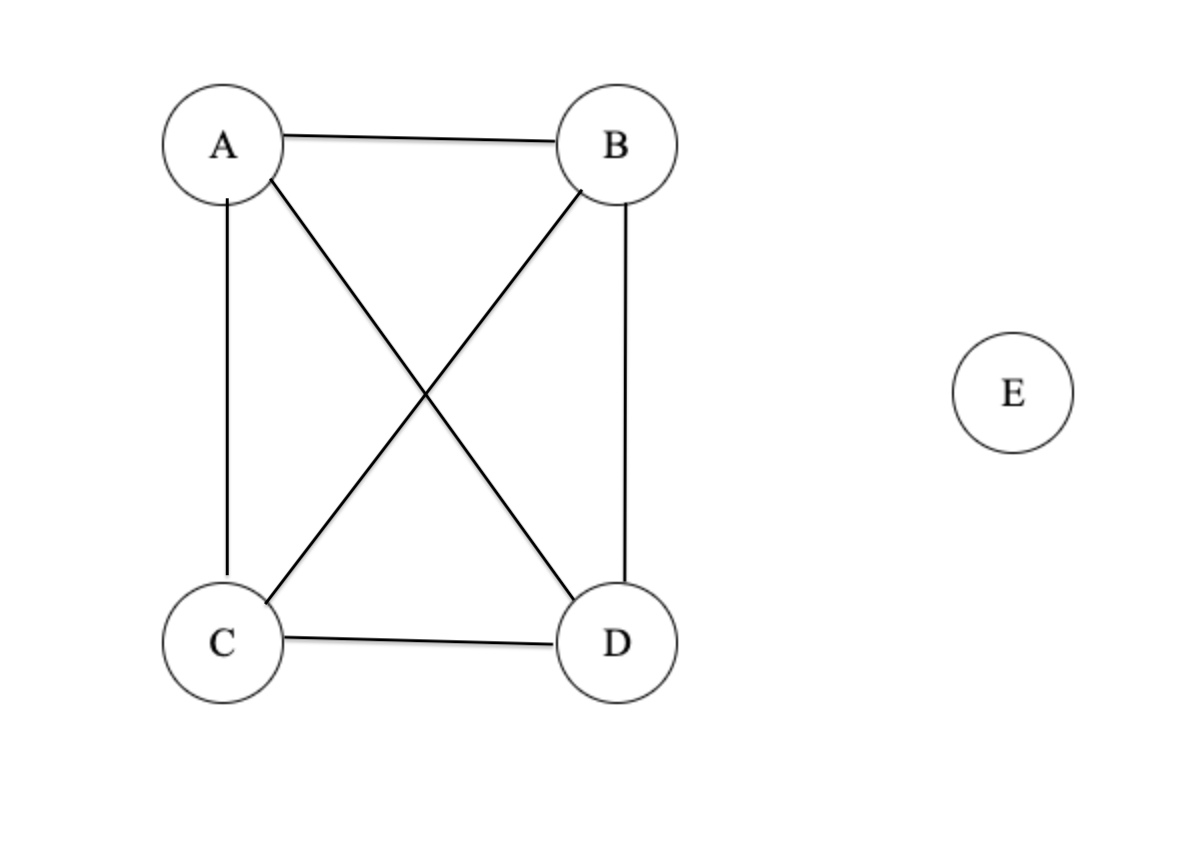
\includegraphics[width=8cm]{partc.png}
    \caption{Disconnected Undirected Graph}
    \label{fig:tree}
\end{figure}


\end{enumerate}

\end{document}